\documentclass[1p]{elsarticle_modified}
%\bibliographystyle{elsarticle-num}

%\usepackage[colorlinks]{hyperref}
%\usepackage{abbrmath_seonhwa} %\Abb, \Ascr, \Acal ,\Abf, \Afrak
\usepackage{amsfonts}
\usepackage{amssymb}
\usepackage{amsmath}
\usepackage{amsthm}
\usepackage{scalefnt}
\usepackage{amsbsy}
\usepackage{kotex}
\usepackage{caption}
\usepackage{subfig}
\usepackage{color}
\usepackage{graphicx}
\usepackage{xcolor} %% white, black, red, green, blue, cyan, magenta, yellow
\usepackage{float}
\usepackage{setspace}
\usepackage{hyperref}

\usepackage{tikz}
\usetikzlibrary{arrows}

\usepackage{multirow}
\usepackage{array} % fixed length table
\usepackage{hhline}

%%%%%%%%%%%%%%%%%%%%%
\makeatletter
\renewcommand*\env@matrix[1][\arraystretch]{%
	\edef\arraystretch{#1}%
	\hskip -\arraycolsep
	\let\@ifnextchar\new@ifnextchar
	\array{*\c@MaxMatrixCols c}}
\makeatother %https://tex.stackexchange.com/questions/14071/how-can-i-increase-the-line-spacing-in-a-matrix
%%%%%%%%%%%%%%%

\usepackage[normalem]{ulem}

\newcommand{\msout}[1]{\ifmmode\text{\sout{\ensuremath{#1}}}\else\sout{#1}\fi}
%SOURCE: \msout is \stkout macro in https://tex.stackexchange.com/questions/20609/strikeout-in-math-mode

\newcommand{\cancel}[1]{
	\ifmmode
	{\color{red}\msout{#1}}
	\else
	{\color{red}\sout{#1}}
	\fi
}

\newcommand{\add}[1]{
	{\color{blue}\uwave{#1}}
}

\newcommand{\replace}[2]{
	\ifmmode
	{\color{red}\msout{#1}}{\color{blue}\uwave{#2}}
	\else
	{\color{red}\sout{#1}}{\color{blue}\uwave{#2}}
	\fi
}

\newcommand{\Sol}{\mathcal{S}} %segment
\newcommand{\D}{D} %diagram
\newcommand{\A}{\mathcal{A}} %arc


%%%%%%%%%%%%%%%%%%%%%%%%%%%%%5 test

\def\sl{\operatorname{\textup{SL}}(2,\Cbb)}
\def\psl{\operatorname{\textup{PSL}}(2,\Cbb)}
\def\quan{\mkern 1mu \triangleright \mkern 1mu}

\theoremstyle{definition}
\newtheorem{thm}{Theorem}[section]
\newtheorem{prop}[thm]{Proposition}
\newtheorem{lem}[thm]{Lemma}
\newtheorem{ques}[thm]{Question}
\newtheorem{cor}[thm]{Corollary}
\newtheorem{defn}[thm]{Definition}
\newtheorem{exam}[thm]{Example}
\newtheorem{rmk}[thm]{Remark}
\newtheorem{alg}[thm]{Algorithm}

\newcommand{\I}{\sqrt{-1}}
\begin{document}

%\begin{frontmatter}
%
%\title{Boundary parabolic representations of knots up to 8 crossings}
%
%%% Group authors per affiliation:
%\author{Yunhi Cho} 
%\address{Department of Mathematics, University of Seoul, Seoul, Korea}
%\ead{yhcho@uos.ac.kr}
%
%
%\author{Seonhwa Kim} %\fnref{s_kim}}
%\address{Center for Geometry and Physics, Institute for Basic Science, Pohang, 37673, Korea}
%\ead{ryeona17@ibs.re.kr}
%
%\author{Hyuk Kim}
%\address{Department of Mathematical Sciences, Seoul National University, Seoul 08826, Korea}
%\ead{hyukkim@snu.ac.kr}
%
%\author{Seokbeom Yoon}
%\address{Department of Mathematical Sciences, Seoul National University, Seoul, 08826,  Korea}
%\ead{sbyoon15@snu.ac.kr}
%
%\begin{abstract}
%We find all boundary parabolic representation of knots up to 8 crossings.
%
%\end{abstract}
%\begin{keyword}
%    \MSC[2010] 57M25 
%\end{keyword}
%
%\end{frontmatter}

%\linenumbers
%\tableofcontents
%
\newcommand\colored[1]{\textcolor{white}{\rule[-0.35ex]{0.8em}{1.4ex}}\kern-0.8em\color{red} #1}%
%\newcommand\colored[1]{\textcolor{white}{ #1}\kern-2.17ex	\textcolor{white}{ #1}\kern-1.81ex	\textcolor{white}{ #1}\kern-2.15ex\color{red}#1	}

{\Large $\underline{12n_{0751}~(K12n_{0751})}$}

\setlength{\tabcolsep}{10pt}
\renewcommand{\arraystretch}{1.6}
\vspace{1cm}\begin{tabular}{m{100pt}>{\centering\arraybackslash}m{274pt}}
\multirow{5}{120pt}{
	\centering
	\includegraphics[width=112pt]{../../../GIT/diagram.site/Diagrams/png/2840_12n_0751.png}\\
\ \ \ A knot diagram\footnotemark}&
\allowdisplaybreaks
\textbf{Linearized knot diagam} \\
\cline{2-2}
 &
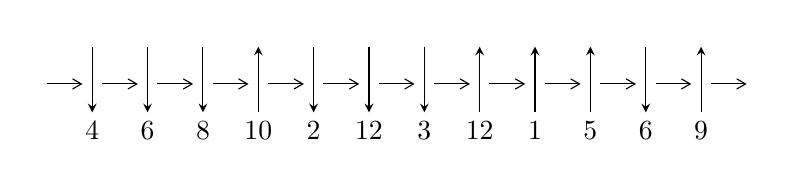
\begin{tikzpicture}[x=20pt, y=17pt]
	% nodes
	\node (C0) at (0, 0) {};
	\node (C1) at (1, 0) {};
	\node (C1U) at (1, +1) {};
	\node (C1D) at (1, -1) {4};

	\node (C2) at (2, 0) {};
	\node (C2U) at (2, +1) {};
	\node (C2D) at (2, -1) {6};

	\node (C3) at (3, 0) {};
	\node (C3U) at (3, +1) {};
	\node (C3D) at (3, -1) {8};

	\node (C4) at (4, 0) {};
	\node (C4U) at (4, +1) {};
	\node (C4D) at (4, -1) {10};

	\node (C5) at (5, 0) {};
	\node (C5U) at (5, +1) {};
	\node (C5D) at (5, -1) {2};

	\node (C6) at (6, 0) {};
	\node (C6U) at (6, +1) {};
	\node (C6D) at (6, -1) {12};

	\node (C7) at (7, 0) {};
	\node (C7U) at (7, +1) {};
	\node (C7D) at (7, -1) {3};

	\node (C8) at (8, 0) {};
	\node (C8U) at (8, +1) {};
	\node (C8D) at (8, -1) {12};

	\node (C9) at (9, 0) {};
	\node (C9U) at (9, +1) {};
	\node (C9D) at (9, -1) {1};

	\node (C10) at (10, 0) {};
	\node (C10U) at (10, +1) {};
	\node (C10D) at (10, -1) {5};

	\node (C11) at (11, 0) {};
	\node (C11U) at (11, +1) {};
	\node (C11D) at (11, -1) {6};

	\node (C12) at (12, 0) {};
	\node (C12U) at (12, +1) {};
	\node (C12D) at (12, -1) {9};
	\node (C13) at (13, 0) {};

	% arrows
	\draw[->,>={angle 60}]
	(C0) edge (C1) (C1) edge (C2) (C2) edge (C3) (C3) edge (C4) (C4) edge (C5) (C5) edge (C6) (C6) edge (C7) (C7) edge (C8) (C8) edge (C9) (C9) edge (C10) (C10) edge (C11) (C11) edge (C12) (C12) edge (C13) ;	\draw[->,>=stealth]
	(C1U) edge (C1D) (C2U) edge (C2D) (C3U) edge (C3D) (C4D) edge (C4U) (C5U) edge (C5D) (C6U) edge (C6D) (C7U) edge (C7D) (C8D) edge (C8U) (C9D) edge (C9U) (C10D) edge (C10U) (C11U) edge (C11D) (C12D) edge (C12U) ;
	\end{tikzpicture} \\
\hhline{~~} \\& 
\textbf{Solving Sequence} \\ \cline{2-2} 
 &
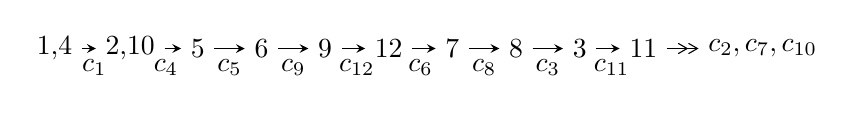
\begin{tikzpicture}[x=23pt, y=7pt]
	% node
	\node (A0) at (-1/8, 0) {1,4};
	\node (A1) at (17/16, 0) {2,10};
	\node (A2) at (17/8, 0) {5};
	\node (A3) at (25/8, 0) {6};
	\node (A4) at (33/8, 0) {9};
	\node (A5) at (41/8, 0) {12};
	\node (A6) at (49/8, 0) {7};
	\node (A7) at (57/8, 0) {8};
	\node (A8) at (65/8, 0) {3};
	\node (A9) at (73/8, 0) {11};
	\node (C1) at (1/2, -1) {$c_{1}$};
	\node (C2) at (13/8, -1) {$c_{4}$};
	\node (C3) at (21/8, -1) {$c_{5}$};
	\node (C4) at (29/8, -1) {$c_{9}$};
	\node (C5) at (37/8, -1) {$c_{12}$};
	\node (C6) at (45/8, -1) {$c_{6}$};
	\node (C7) at (53/8, -1) {$c_{8}$};
	\node (C8) at (61/8, -1) {$c_{3}$};
	\node (C9) at (69/8, -1) {$c_{11}$};
	\node (A10) at (11, 0) {$c_{2},c_{7},c_{10}$};

	% edge
	\draw[->,>=stealth]	
	(A0) edge (A1) (A1) edge (A2) (A2) edge (A3) (A3) edge (A4) (A4) edge (A5) (A5) edge (A6) (A6) edge (A7) (A7) edge (A8) (A8) edge (A9) ;
	\draw[->>,>={angle 60}]	
	(A9) edge (A10);
\end{tikzpicture} \\ 

\end{tabular} \\

\footnotetext{
The image of knot diagram is generated by the software ``\textbf{Draw programme}" developed by Andrew Bartholomew(\url{http://www.layer8.co.uk/maths/draw/index.htm\#Running-draw}), where we modified some parts for our purpose(\url{https://github.com/CATsTAILs/LinksPainter}).
}\phantom \\ \newline 
\centering \textbf{Ideals for irreducible components\footnotemark of $X_{\text{par}}$} 
 
\begin{align*}
I^u_{1}&=\langle 
-898244027 u^{14}-391531130 u^{13}+\cdots+534701171 b+1119066057,\\
\phantom{I^u_{1}}&\phantom{= \langle  }-898027536 u^{14}-389544550 u^{13}+\cdots+534701171 a+1652680736,\\
\phantom{I^u_{1}}&\phantom{= \langle  }u^{15}- u^{13}- u^{12}+8 u^{11}- u^{10}-18 u^9-2 u^7+12 u^6-21 u^5+26 u^4-14 u^3+3 u^2-2 u+1\rangle \\
I^u_{2}&=\langle 
3.30670\times10^{41} u^{29}+5.71881\times10^{41} u^{28}+\cdots+1.78529\times10^{43} b+3.34070\times10^{43},\\
\phantom{I^u_{2}}&\phantom{= \langle  }1.36375\times10^{44} u^{29}-4.57521\times10^{43} u^{28}+\cdots+3.92765\times10^{44} a+3.57143\times10^{45},\;u^{30}+2 u^{28}+\cdots+81 u+11\rangle \\
I^u_{3}&=\langle 
u^3+b+3,\;u^3+a- u+2,\;u^4+u^3+2 u+1\rangle \\
I^u_{4}&=\langle 
b,\;a+u-2,\;u^2- u-1\rangle \\
I^u_{5}&=\langle 
u^2+b- u-1,\;- u^3+2 u^2+a+u-1,\;u^4-2 u^3- u^2+2 u-1\rangle \\
I^u_{6}&=\langle 
b,\;a-1,\;u-1\rangle \\
I^u_{7}&=\langle 
b-1,\;a^2- a-1,\;u-1\rangle \\
\\
\end{align*}
\raggedright * 7 irreducible components of $\dim_{\mathbb{C}}=0$, with total 58 representations.\\
\footnotetext{All coefficients of polynomials are rational numbers. But the coefficients are sometimes approximated in decimal forms when there is not enough margin.}
\newpage
\renewcommand{\arraystretch}{1}
\centering \section*{I. $I^u_{1}= \langle -8.98\times10^{8} u^{14}-3.92\times10^{8} u^{13}+\cdots+5.35\times10^{8} b+1.12\times10^{9},\;-8.98\times10^{8} u^{14}-3.90\times10^{8} u^{13}+\cdots+5.35\times10^{8} a+1.65\times10^{9},\;u^{15}- u^{13}+\cdots-2 u+1 \rangle$}
\flushleft \textbf{(i) Arc colorings}\\
\begin{tabular}{m{7pt} m{180pt} m{7pt} m{180pt} }
\flushright $a_{1}=$&$\begin{pmatrix}1\\0\end{pmatrix}$ \\
\flushright $a_{4}=$&$\begin{pmatrix}0\\u\end{pmatrix}$ \\
\flushright $a_{2}=$&$\begin{pmatrix}1\\u^2\end{pmatrix}$ \\
\flushright $a_{10}=$&$\begin{pmatrix}1.67949 u^{14}+0.728528 u^{13}+\cdots+3.65635 u-3.09085\\1.67990 u^{14}+0.732243 u^{13}+\cdots+0.801226 u-2.09288\end{pmatrix}$ \\
\flushright $a_{5}=$&$\begin{pmatrix}-1.07086 u^{14}-0.594830 u^{13}+\cdots-2.20938 u+2.32522\\-1.79456 u^{14}-0.830294 u^{13}+\cdots-0.599907 u+2.64579\end{pmatrix}$ \\
\flushright $a_{6}=$&$\begin{pmatrix}0.235869 u^{14}-0.0456390 u^{13}+\cdots-1.72828 u+0.274259\\-1.49103 u^{14}-0.606558 u^{13}+\cdots-0.808252 u+2.09660\end{pmatrix}$ \\
\flushright $a_{9}=$&$\begin{pmatrix}-0.000404882 u^{14}-0.00371531 u^{13}+\cdots+2.85513 u-0.997968\\1.67990 u^{14}+0.732243 u^{13}+\cdots+0.801226 u-2.09288\end{pmatrix}$ \\
\flushright $a_{12}=$&$\begin{pmatrix}-0.000404882 u^{14}-0.00371531 u^{13}+\cdots+2.85513 u-0.997968\\-2.64538 u^{14}-1.79085 u^{13}+\cdots+0.108289 u+5.68964\end{pmatrix}$ \\
\flushright $a_{7}=$&$\begin{pmatrix}u^2-1\\4.04447 u^{14}+2.08478 u^{13}+\cdots+5.22270 u-7.34077\end{pmatrix}$ \\
\flushright $a_{8}=$&$\begin{pmatrix}1\\-5.94603 u^{14}-3.12181 u^{13}+\cdots-5.52030 u+10.4626\end{pmatrix}$ \\
\flushright $a_{3}=$&$\begin{pmatrix}u\\-3.12181 u^{14}-1.90156 u^{13}+\cdots-0.429474 u+5.94603\end{pmatrix}$ \\
\flushright $a_{11}=$&$\begin{pmatrix}0.209193 u^{14}-0.0694314 u^{13}+\cdots+1.83397 u-0.107940\\-0.645989 u^{14}-0.381117 u^{13}+\cdots-0.616195 u+1.74893\end{pmatrix}$\\&\end{tabular}
\flushleft \textbf{(ii) Obstruction class $= -1$}\\~\\
\flushleft \textbf{(iii) Cusp Shapes $= -\frac{9257204513}{534701171} u^{14}-\frac{6026834044}{534701171} u^{13}+\cdots-\frac{11292543056}{534701171} u+\frac{18370247823}{534701171}$}\\~\\
\newpage\renewcommand{\arraystretch}{1}
\flushleft \textbf{(iv) u-Polynomials at the component}\newline \\
\begin{tabular}{m{50pt}|m{274pt}}
Crossings & \hspace{64pt}u-Polynomials at each crossing \\
\hline $$\begin{aligned}c_{1},c_{3},c_{7}\end{aligned}$$&$\begin{aligned}
&u^{15}- u^{13}+\cdots-2 u-1
\end{aligned}$\\
\hline $$\begin{aligned}c_{2},c_{5}\end{aligned}$$&$\begin{aligned}
&u^{15}+9 u^{14}+\cdots-69 u-9
\end{aligned}$\\
\hline $$\begin{aligned}c_{4},c_{10}\end{aligned}$$&$\begin{aligned}
&u^{15}- u^{14}+\cdots+5 u+1
\end{aligned}$\\
\hline $$\begin{aligned}c_{6},c_{11}\end{aligned}$$&$\begin{aligned}
&u^{15}- u^{14}+\cdots-4 u-1
\end{aligned}$\\
\hline $$\begin{aligned}c_{8},c_{9},c_{12}\end{aligned}$$&$\begin{aligned}
&u^{15}-6 u^{14}+\cdots+6 u+9
\end{aligned}$\\
\hline
\end{tabular}\\~\\
\newpage\renewcommand{\arraystretch}{1}
\flushleft \textbf{(v) Riley Polynomials at the component}\newline \\
\begin{tabular}{m{50pt}|m{274pt}}
Crossings & \hspace{64pt}Riley Polynomials at each crossing \\
\hline $$\begin{aligned}c_{1},c_{3},c_{7}\end{aligned}$$&$\begin{aligned}
&y^{15}-2 y^{14}+\cdots-2 y-1
\end{aligned}$\\
\hline $$\begin{aligned}c_{2},c_{5}\end{aligned}$$&$\begin{aligned}
&y^{15}-9 y^{14}+\cdots+1071 y-81
\end{aligned}$\\
\hline $$\begin{aligned}c_{4},c_{10}\end{aligned}$$&$\begin{aligned}
&y^{15}-13 y^{14}+\cdots+39 y-1
\end{aligned}$\\
\hline $$\begin{aligned}c_{6},c_{11}\end{aligned}$$&$\begin{aligned}
&y^{15}+13 y^{14}+\cdots+16 y-1
\end{aligned}$\\
\hline $$\begin{aligned}c_{8},c_{9},c_{12}\end{aligned}$$&$\begin{aligned}
&y^{15}-26 y^{14}+\cdots-1494 y-81
\end{aligned}$\\
\hline
\end{tabular}\\~\\
\newpage\flushleft \textbf{(vi) Complex Volumes and Cusp Shapes}
$$\begin{array}{c|c|c}  
\text{Solutions to }I^u_{1}& \I (\text{vol} + \sqrt{-1}CS) & \text{Cusp shape}\\
 \hline 
\begin{aligned}
u &= \phantom{-}0.219964 + 0.819481 I \\
a &= -1.44756 - 0.16891 I \\
b &= \phantom{-}1.355710 - 0.019020 I\end{aligned}
 & \phantom{-}3.27965 - 1.21970 I & \phantom{-}1.31129 + 5.66741 I \\ \hline\begin{aligned}
u &= \phantom{-}0.219964 - 0.819481 I \\
a &= -1.44756 + 0.16891 I \\
b &= \phantom{-}1.355710 + 0.019020 I\end{aligned}
 & \phantom{-}3.27965 + 1.21970 I & \phantom{-}1.31129 - 5.66741 I \\ \hline\begin{aligned}
u &= -0.788509 + 0.905745 I \\
a &= -0.457133 - 1.143780 I \\
b &= -0.883513 - 0.932651 I\end{aligned}
 & \phantom{-}5.92156 + 9.44163 I & \phantom{-}0.20634 - 8.15923 I \\ \hline\begin{aligned}
u &= -0.788509 - 0.905745 I \\
a &= -0.457133 + 1.143780 I \\
b &= -0.883513 + 0.932651 I\end{aligned}
 & \phantom{-}5.92156 - 9.44163 I & \phantom{-}0.20634 + 8.15923 I \\ \hline\begin{aligned}
u &= \phantom{-}0.623880 + 0.248532 I \\
a &= \phantom{-}0.809525 + 0.462868 I \\
b &= -0.072998 + 0.253976 I\end{aligned}
 & -1.140580 - 0.339277 I & -8.98924 + 1.73624 I \\ \hline\begin{aligned}
u &= \phantom{-}0.623880 - 0.248532 I \\
a &= \phantom{-}0.809525 - 0.462868 I \\
b &= -0.072998 - 0.253976 I\end{aligned}
 & -1.140580 + 0.339277 I & -8.98924 - 1.73624 I \\ \hline\begin{aligned}
u &= \phantom{-}0.565700\phantom{ +0.000000I} \\
a &= -2.01244\phantom{ +0.000000I} \\
b &= -2.31417\phantom{ +0.000000I}\end{aligned}
 & \phantom{-}3.82898\phantom{ +0.000000I} & \phantom{-}27.9490\phantom{ +0.000000I} \\ \hline\begin{aligned}
u &= \phantom{-}1.44661\phantom{ +0.000000I} \\
a &= -0.971679\phantom{ +0.000000I} \\
b &= -1.39008\phantom{ +0.000000I}\end{aligned}
 & \phantom{-}3.06003\phantom{ +0.000000I} & \phantom{-}2.95830\phantom{ +0.000000I} \\ \hline\begin{aligned}
u &= -1.52296\phantom{ +0.000000I} \\
a &= -0.111508\phantom{ +0.000000I} \\
b &= -0.699810\phantom{ +0.000000I}\end{aligned}
 & -7.76254\phantom{ +0.000000I} & -32.3850\phantom{ +0.000000I} \\ \hline\begin{aligned}
u &= -0.192664 + 0.382554 I \\
a &= \phantom{-}0.23984 + 1.65841 I \\
b &= \phantom{-}1.40585 + 0.42820 I\end{aligned}
 & \phantom{-}2.17147 + 0.68609 I & \phantom{-}8.04360 - 5.02078 I\\
 \hline 
 \end{array}$$\newpage$$\begin{array}{c|c|c}  
\text{Solutions to }I^u_{1}& \I (\text{vol} + \sqrt{-1}CS) & \text{Cusp shape}\\
 \hline 
\begin{aligned}
u &= -0.192664 - 0.382554 I \\
a &= \phantom{-}0.23984 - 1.65841 I \\
b &= \phantom{-}1.40585 - 0.42820 I\end{aligned}
 & \phantom{-}2.17147 - 0.68609 I & \phantom{-}8.04360 + 5.02078 I \\ \hline\begin{aligned}
u &= \phantom{-}1.10259 + 1.29441 I \\
a &= \phantom{-}0.497805 - 0.641547 I \\
b &= \phantom{-}1.73219 - 0.23886 I\end{aligned}
 & \phantom{-}14.6227 - 4.7692 I & \phantom{-}3.20527 + 2.44636 I \\ \hline\begin{aligned}
u &= \phantom{-}1.10259 - 1.29441 I \\
a &= \phantom{-}0.497805 + 0.641547 I \\
b &= \phantom{-}1.73219 + 0.23886 I\end{aligned}
 & \phantom{-}14.6227 + 4.7692 I & \phantom{-}3.20527 - 2.44636 I \\ \hline\begin{aligned}
u &= -1.20993 + 1.32914 I \\
a &= \phantom{-}0.405328 + 0.848334 I \\
b &= \phantom{-}1.66478 + 0.29308 I\end{aligned}
 & \phantom{-}14.2379 + 14.0822 I & \phantom{-}1.96139 - 6.46819 I \\ \hline\begin{aligned}
u &= -1.20993 - 1.32914 I \\
a &= \phantom{-}0.405328 - 0.848334 I \\
b &= \phantom{-}1.66478 - 0.29308 I\end{aligned}
 & \phantom{-}14.2379 - 14.0822 I & \phantom{-}1.96139 + 6.46819 I\\
 \hline 
 \end{array}$$\newpage\newpage\renewcommand{\arraystretch}{1}
\centering \section*{II. $I^u_{2}= \langle 3.31\times10^{41} u^{29}+5.72\times10^{41} u^{28}+\cdots+1.79\times10^{43} b+3.34\times10^{43},\;1.36\times10^{44} u^{29}-4.58\times10^{43} u^{28}+\cdots+3.93\times10^{44} a+3.57\times10^{45},\;u^{30}+2 u^{28}+\cdots+81 u+11 \rangle$}
\flushleft \textbf{(i) Arc colorings}\\
\begin{tabular}{m{7pt} m{180pt} m{7pt} m{180pt} }
\flushright $a_{1}=$&$\begin{pmatrix}1\\0\end{pmatrix}$ \\
\flushright $a_{4}=$&$\begin{pmatrix}0\\u\end{pmatrix}$ \\
\flushright $a_{2}=$&$\begin{pmatrix}1\\u^2\end{pmatrix}$ \\
\flushright $a_{10}=$&$\begin{pmatrix}-0.347218 u^{29}+0.116487 u^{28}+\cdots-51.0446 u-9.09305\\-0.0185219 u^{29}-0.0320329 u^{28}+\cdots-11.9126 u-1.87123\end{pmatrix}$ \\
\flushright $a_{5}=$&$\begin{pmatrix}-0.394706 u^{29}+0.210595 u^{28}+\cdots-41.4801 u-8.32205\\-0.0263285 u^{29}+0.0298042 u^{28}+\cdots+6.05343 u+1.54652\end{pmatrix}$ \\
\flushright $a_{6}=$&$\begin{pmatrix}-0.467058 u^{29}+0.222944 u^{28}+\cdots-60.2499 u-12.1851\\-0.0503337 u^{29}+0.0560610 u^{28}+\cdots+5.84906 u+1.41068\end{pmatrix}$ \\
\flushright $a_{9}=$&$\begin{pmatrix}-0.328697 u^{29}+0.148520 u^{28}+\cdots-39.1319 u-7.22182\\-0.0185219 u^{29}-0.0320329 u^{28}+\cdots-11.9126 u-1.87123\end{pmatrix}$ \\
\flushright $a_{12}=$&$\begin{pmatrix}-0.196754 u^{29}+0.0387220 u^{28}+\cdots-27.9600 u-3.50095\\0.0561620 u^{29}-0.0650505 u^{28}+\cdots-7.03644 u-1.83361\end{pmatrix}$ \\
\flushright $a_{7}=$&$\begin{pmatrix}-0.409410 u^{29}+0.0902696 u^{28}+\cdots-81.9335 u-16.7607\\0.0570621 u^{29}+0.0581006 u^{28}+\cdots+19.7385 u+2.64502\end{pmatrix}$ \\
\flushright $a_{8}=$&$\begin{pmatrix}-0.217120 u^{29}+0.141042 u^{28}+\cdots-12.8730 u-3.08396\\-0.0595359 u^{29}+0.0111266 u^{28}+\cdots-9.03611 u-0.551467\end{pmatrix}$ \\
\flushright $a_{3}=$&$\begin{pmatrix}-0.562677 u^{29}+0.183364 u^{28}+\cdots-77.5261 u-13.9939\\0.105143 u^{29}-0.0492747 u^{28}+\cdots+6.83973 u+0.371317\end{pmatrix}$ \\
\flushright $a_{11}=$&$\begin{pmatrix}0.209727 u^{29}-0.119739 u^{28}+\cdots+27.3054 u+6.97658\\-0.0548665 u^{29}-0.0623507 u^{28}+\cdots-18.5446 u-2.63799\end{pmatrix}$\\&\end{tabular}
\flushleft \textbf{(ii) Obstruction class $= -1$}\\~\\
\flushleft \textbf{(iii) Cusp Shapes $= 0.347221 u^{29}-0.0667960 u^{28}+\cdots+55.5079 u+14.9386$}\\~\\
\newpage\renewcommand{\arraystretch}{1}
\flushleft \textbf{(iv) u-Polynomials at the component}\newline \\
\begin{tabular}{m{50pt}|m{274pt}}
Crossings & \hspace{64pt}u-Polynomials at each crossing \\
\hline $$\begin{aligned}c_{1},c_{3},c_{7}\end{aligned}$$&$\begin{aligned}
&u^{30}+2 u^{28}+\cdots-81 u+11
\end{aligned}$\\
\hline $$\begin{aligned}c_{2},c_{5}\end{aligned}$$&$\begin{aligned}
&(u^{15}-4 u^{14}+\cdots-5 u+2)^{2}
\end{aligned}$\\
\hline $$\begin{aligned}c_{4},c_{10}\end{aligned}$$&$\begin{aligned}
&u^{30}- u^{29}+\cdots-24 u+1
\end{aligned}$\\
\hline $$\begin{aligned}c_{6},c_{11}\end{aligned}$$&$\begin{aligned}
&u^{30}+2 u^{29}+\cdots+31 u+1
\end{aligned}$\\
\hline $$\begin{aligned}c_{8},c_{9},c_{12}\end{aligned}$$&$\begin{aligned}
&(u^{15}+2 u^{14}+\cdots-2 u+2)^{2}
\end{aligned}$\\
\hline
\end{tabular}\\~\\
\newpage\renewcommand{\arraystretch}{1}
\flushleft \textbf{(v) Riley Polynomials at the component}\newline \\
\begin{tabular}{m{50pt}|m{274pt}}
Crossings & \hspace{64pt}Riley Polynomials at each crossing \\
\hline $$\begin{aligned}c_{1},c_{3},c_{7}\end{aligned}$$&$\begin{aligned}
&y^{30}+4 y^{29}+\cdots+105 y+121
\end{aligned}$\\
\hline $$\begin{aligned}c_{2},c_{5}\end{aligned}$$&$\begin{aligned}
&(y^{15}+8 y^{13}+\cdots-3 y-4)^{2}
\end{aligned}$\\
\hline $$\begin{aligned}c_{4},c_{10}\end{aligned}$$&$\begin{aligned}
&y^{30}-33 y^{29}+\cdots-56 y+1
\end{aligned}$\\
\hline $$\begin{aligned}c_{6},c_{11}\end{aligned}$$&$\begin{aligned}
&y^{30}+26 y^{29}+\cdots-177 y+1
\end{aligned}$\\
\hline $$\begin{aligned}c_{8},c_{9},c_{12}\end{aligned}$$&$\begin{aligned}
&(y^{15}-18 y^{14}+\cdots+68 y-4)^{2}
\end{aligned}$\\
\hline
\end{tabular}\\~\\
\newpage\flushleft \textbf{(vi) Complex Volumes and Cusp Shapes}
$$\begin{array}{c|c|c}  
\text{Solutions to }I^u_{2}& \I (\text{vol} + \sqrt{-1}CS) & \text{Cusp shape}\\
 \hline 
\begin{aligned}
u &= -0.975339\phantom{ +0.000000I} \\
a &= \phantom{-}2.03736\phantom{ +0.000000I} \\
b &= \phantom{-}1.13495\phantom{ +0.000000I}\end{aligned}
 & -0.455497\phantom{ +0.000000I} & -13.6410\phantom{ +0.000000I} \\ \hline\begin{aligned}
u &= \phantom{-}0.962045 + 0.405621 I \\
a &= -0.920194 + 0.526296 I \\
b &= -1.53636\phantom{ +0.000000I}\end{aligned}
 & \phantom{-}3.54960\phantom{ +0.000000I} & \phantom{-}2.31783 + 0. I\phantom{ +0.000000I} \\ \hline\begin{aligned}
u &= \phantom{-}0.962045 - 0.405621 I \\
a &= -0.920194 - 0.526296 I \\
b &= -1.53636\phantom{ +0.000000I}\end{aligned}
 & \phantom{-}3.54960\phantom{ +0.000000I} & \phantom{-}2.31783 + 0. I\phantom{ +0.000000I} \\ \hline\begin{aligned}
u &= -0.605280 + 0.637023 I \\
a &= \phantom{-}0.47688 - 1.78582 I \\
b &= -1.47359 - 0.25718 I\end{aligned}
 & \phantom{-}6.96654 + 7.44645 I & -1.97655 - 7.47153 I \\ \hline\begin{aligned}
u &= -0.605280 - 0.637023 I \\
a &= \phantom{-}0.47688 + 1.78582 I \\
b &= -1.47359 + 0.25718 I\end{aligned}
 & \phantom{-}6.96654 - 7.44645 I & -1.97655 + 7.47153 I \\ \hline\begin{aligned}
u &= \phantom{-}0.518757 + 0.995170 I \\
a &= \phantom{-}0.188630 - 0.965072 I \\
b &= \phantom{-}0.398627 - 0.770277 I\end{aligned}
 & \phantom{-}0.92420 - 3.75884 I & -2.83571 + 8.62550 I \\ \hline\begin{aligned}
u &= \phantom{-}0.518757 - 0.995170 I \\
a &= \phantom{-}0.188630 + 0.965072 I \\
b &= \phantom{-}0.398627 + 0.770277 I\end{aligned}
 & \phantom{-}0.92420 + 3.75884 I & -2.83571 - 8.62550 I \\ \hline\begin{aligned}
u &= \phantom{-}0.508270 + 1.021130 I \\
a &= -0.311123 + 1.376970 I \\
b &= -0.566489 + 0.063512 I\end{aligned}
 & \phantom{-}6.65494 - 3.78113 I & \phantom{-}2.84579 + 3.30508 I \\ \hline\begin{aligned}
u &= \phantom{-}0.508270 - 1.021130 I \\
a &= -0.311123 - 1.376970 I \\
b &= -0.566489 - 0.063512 I\end{aligned}
 & \phantom{-}6.65494 + 3.78113 I & \phantom{-}2.84579 - 3.30508 I \\ \hline\begin{aligned}
u &= -0.069702 + 1.177270 I \\
a &= \phantom{-}0.0457627 + 0.0466319 I \\
b &= -1.61515 + 0.17952 I\end{aligned}
 & \phantom{-}9.74746 - 4.20828 I & \phantom{-}3.86853 + 1.95225 I\\
 \hline 
 \end{array}$$\newpage$$\begin{array}{c|c|c}  
\text{Solutions to }I^u_{2}& \I (\text{vol} + \sqrt{-1}CS) & \text{Cusp shape}\\
 \hline 
\begin{aligned}
u &= -0.069702 - 1.177270 I \\
a &= \phantom{-}0.0457627 - 0.0466319 I \\
b &= -1.61515 - 0.17952 I\end{aligned}
 & \phantom{-}9.74746 + 4.20828 I & \phantom{-}3.86853 - 1.95225 I \\ \hline\begin{aligned}
u &= -0.541567 + 1.093190 I \\
a &= -0.672453 - 0.922756 I \\
b &= -0.566489 + 0.063512 I\end{aligned}
 & \phantom{-}6.65494 - 3.78113 I & \phantom{-}2.84579 + 3.30508 I \\ \hline\begin{aligned}
u &= -0.541567 - 1.093190 I \\
a &= -0.672453 + 0.922756 I \\
b &= -0.566489 - 0.063512 I\end{aligned}
 & \phantom{-}6.65494 + 3.78113 I & \phantom{-}2.84579 - 3.30508 I \\ \hline\begin{aligned}
u &= -0.661146 + 0.389686 I \\
a &= -0.48702 + 1.46762 I \\
b &= \phantom{-}0.398627 + 0.770277 I\end{aligned}
 & \phantom{-}0.92420 + 3.75884 I & -2.83571 - 8.62550 I \\ \hline\begin{aligned}
u &= -0.661146 - 0.389686 I \\
a &= -0.48702 - 1.46762 I \\
b &= \phantom{-}0.398627 - 0.770277 I\end{aligned}
 & \phantom{-}0.92420 - 3.75884 I & -2.83571 + 8.62550 I \\ \hline\begin{aligned}
u &= -0.307321 + 0.642721 I \\
a &= \phantom{-}0.30958 + 1.50914 I \\
b &= \phantom{-}0.709925 + 0.664105 I\end{aligned}
 & \phantom{-}1.88098 + 1.11902 I & \phantom{-}2.92830 + 0.60819 I \\ \hline\begin{aligned}
u &= -0.307321 - 0.642721 I \\
a &= \phantom{-}0.30958 - 1.50914 I \\
b &= \phantom{-}0.709925 - 0.664105 I\end{aligned}
 & \phantom{-}1.88098 - 1.11902 I & \phantom{-}2.92830 - 0.60819 I \\ \hline\begin{aligned}
u &= \phantom{-}1.36054\phantom{ +0.000000I} \\
a &= -0.316147\phantom{ +0.000000I} \\
b &= \phantom{-}1.13495\phantom{ +0.000000I}\end{aligned}
 & -0.455497\phantom{ +0.000000I} & -13.6410\phantom{ +0.000000I} \\ \hline\begin{aligned}
u &= -0.429729\phantom{ +0.000000I} \\
a &= -3.56723\phantom{ +0.000000I} \\
b &= \phantom{-}0.336879\phantom{ +0.000000I}\end{aligned}
 & -3.04205\phantom{ +0.000000I} & \phantom{-}11.2360\phantom{ +0.000000I} \\ \hline\begin{aligned}
u &= -0.236133 + 0.340530 I \\
a &= \phantom{-}1.077030 - 0.148667 I \\
b &= \phantom{-}0.709925 - 0.664105 I\end{aligned}
 & \phantom{-}1.88098 - 1.11902 I & \phantom{-}2.92830 - 0.60819 I\\
 \hline 
 \end{array}$$\newpage$$\begin{array}{c|c|c}  
\text{Solutions to }I^u_{2}& \I (\text{vol} + \sqrt{-1}CS) & \text{Cusp shape}\\
 \hline 
\begin{aligned}
u &= -0.236133 - 0.340530 I \\
a &= \phantom{-}1.077030 + 0.148667 I \\
b &= \phantom{-}0.709925 + 0.664105 I\end{aligned}
 & \phantom{-}1.88098 + 1.11902 I & \phantom{-}2.92830 + 0.60819 I \\ \hline\begin{aligned}
u &= -1.10466 + 1.15958 I \\
a &= -0.505916 - 0.815295 I \\
b &= -1.61515 - 0.17952 I\end{aligned}
 & \phantom{-}9.74746 + 4.20828 I & \phantom{-}3.86853 - 1.95225 I \\ \hline\begin{aligned}
u &= -1.10466 - 1.15958 I \\
a &= -0.505916 + 0.815295 I \\
b &= -1.61515 + 0.17952 I\end{aligned}
 & \phantom{-}9.74746 - 4.20828 I & \phantom{-}3.86853 + 1.95225 I \\ \hline\begin{aligned}
u &= \phantom{-}1.63208\phantom{ +0.000000I} \\
a &= \phantom{-}0.419875\phantom{ +0.000000I} \\
b &= \phantom{-}0.336879\phantom{ +0.000000I}\end{aligned}
 & -3.04205\phantom{ +0.000000I} & \phantom{-}11.2360\phantom{ +0.000000I} \\ \hline\begin{aligned}
u &= \phantom{-}0.81585 + 1.45626 I \\
a &= -0.089554 + 0.856120 I \\
b &= -1.47359 + 0.25718 I\end{aligned}
 & \phantom{-}6.96654 - 7.44645 I & -2.00000 + 7.47153 I \\ \hline\begin{aligned}
u &= \phantom{-}0.81585 - 1.45626 I \\
a &= -0.089554 - 0.856120 I \\
b &= -1.47359 - 0.25718 I\end{aligned}
 & \phantom{-}6.96654 + 7.44645 I & -2.00000 - 7.47153 I \\ \hline\begin{aligned}
u &= \phantom{-}1.25585 + 1.17832 I \\
a &= \phantom{-}0.577677 - 0.845480 I \\
b &= \phantom{-}1.57894 - 0.03518 I\end{aligned}
 & \phantom{-}14.1007 - 4.2306 I & \phantom{-}2.71313 + 2.44322 I \\ \hline\begin{aligned}
u &= \phantom{-}1.25585 - 1.17832 I \\
a &= \phantom{-}0.577677 + 0.845480 I \\
b &= \phantom{-}1.57894 + 0.03518 I\end{aligned}
 & \phantom{-}14.1007 + 4.2306 I & \phantom{-}2.71313 - 2.44322 I \\ \hline\begin{aligned}
u &= -1.32874 + 1.42818 I \\
a &= \phantom{-}0.478313 + 0.498197 I \\
b &= \phantom{-}1.57894 - 0.03518 I\end{aligned}
 & \phantom{-}14.1007 - 4.2306 I & \phantom{-0.000000 } 0 \\ \hline\begin{aligned}
u &= -1.32874 - 1.42818 I \\
a &= \phantom{-}0.478313 - 0.498197 I \\
b &= \phantom{-}1.57894 + 0.03518 I\end{aligned}
 & \phantom{-}14.1007 + 4.2306 I & \phantom{-0.000000 } 0\\
 \hline 
 \end{array}$$\newpage\newpage\renewcommand{\arraystretch}{1}
\centering \section*{III. $I^u_{3}= \langle u^3+b+3,\;u^3+a- u+2,\;u^4+u^3+2 u+1 \rangle$}
\flushleft \textbf{(i) Arc colorings}\\
\begin{tabular}{m{7pt} m{180pt} m{7pt} m{180pt} }
\flushright $a_{1}=$&$\begin{pmatrix}1\\0\end{pmatrix}$ \\
\flushright $a_{4}=$&$\begin{pmatrix}0\\u\end{pmatrix}$ \\
\flushright $a_{2}=$&$\begin{pmatrix}1\\u^2\end{pmatrix}$ \\
\flushright $a_{10}=$&$\begin{pmatrix}- u^3+u-2\\- u^3-3\end{pmatrix}$ \\
\flushright $a_{5}=$&$\begin{pmatrix}- u^3- u^2- u-3\\-2 u^3-2 u^2+u-3\end{pmatrix}$ \\
\flushright $a_{6}=$&$\begin{pmatrix}- u\\-2 u^3- u^2-3\end{pmatrix}$ \\
\flushright $a_{9}=$&$\begin{pmatrix}u+1\\- u^3-3\end{pmatrix}$ \\
\flushright $a_{12}=$&$\begin{pmatrix}- u-1\\3 u^3+u^2- u+8\end{pmatrix}$ \\
\flushright $a_{7}=$&$\begin{pmatrix}u^2-1\\7 u^3+3 u^2-4 u+15\end{pmatrix}$ \\
\flushright $a_{8}=$&$\begin{pmatrix}-1\\9 u^3+4 u^2-3 u+20\end{pmatrix}$ \\
\flushright $a_{3}=$&$\begin{pmatrix}u\\5 u^3+3 u^2- u+9\end{pmatrix}$ \\
\flushright $a_{11}=$&$\begin{pmatrix}u^3+u^2- u\\- u^2- u+1\end{pmatrix}$\\&\end{tabular}
\flushleft \textbf{(ii) Obstruction class $= 1$}\\~\\
\flushleft \textbf{(iii) Cusp Shapes $= -50 u^3-21 u^2+13 u-97$}\\~\\
\newpage\renewcommand{\arraystretch}{1}
\flushleft \textbf{(iv) u-Polynomials at the component}\newline \\
\begin{tabular}{m{50pt}|m{274pt}}
Crossings & \hspace{64pt}u-Polynomials at each crossing \\
\hline $$\begin{aligned}c_{1},c_{3}\end{aligned}$$&$\begin{aligned}
&u^4+u^3+2 u+1
\end{aligned}$\\
\hline $$\begin{aligned}c_{2}\end{aligned}$$&$\begin{aligned}
&u^4+6 u^3+12 u^2+11 u+5
\end{aligned}$\\
\hline $$\begin{aligned}c_{4}\end{aligned}$$&$\begin{aligned}
&u^4-2 u^3+3 u-1
\end{aligned}$\\
\hline $$\begin{aligned}c_{5}\end{aligned}$$&$\begin{aligned}
&u^4-6 u^3+12 u^2-11 u+5
\end{aligned}$\\
\hline $$\begin{aligned}c_{6}\end{aligned}$$&$\begin{aligned}
&u^4-2 u^3+u^2-4 u-1
\end{aligned}$\\
\hline $$\begin{aligned}c_{7}\end{aligned}$$&$\begin{aligned}
&u^4- u^3-2 u+1
\end{aligned}$\\
\hline $$\begin{aligned}c_{8},c_{9}\end{aligned}$$&$\begin{aligned}
&u^4-5 u^3+6 u^2+2 u-5
\end{aligned}$\\
\hline $$\begin{aligned}c_{10}\end{aligned}$$&$\begin{aligned}
&u^4+2 u^3-3 u-1
\end{aligned}$\\
\hline $$\begin{aligned}c_{11}\end{aligned}$$&$\begin{aligned}
&u^4+2 u^3+u^2+4 u-1
\end{aligned}$\\
\hline $$\begin{aligned}c_{12}\end{aligned}$$&$\begin{aligned}
&u^4+5 u^3+6 u^2-2 u-5
\end{aligned}$\\
\hline
\end{tabular}\\~\\
\newpage\renewcommand{\arraystretch}{1}
\flushleft \textbf{(v) Riley Polynomials at the component}\newline \\
\begin{tabular}{m{50pt}|m{274pt}}
Crossings & \hspace{64pt}Riley Polynomials at each crossing \\
\hline $$\begin{aligned}c_{1},c_{3},c_{7}\end{aligned}$$&$\begin{aligned}
&y^4- y^3-2 y^2-4 y+1
\end{aligned}$\\
\hline $$\begin{aligned}c_{2},c_{5}\end{aligned}$$&$\begin{aligned}
&y^4-12 y^3+22 y^2- y+25
\end{aligned}$\\
\hline $$\begin{aligned}c_{4},c_{10}\end{aligned}$$&$\begin{aligned}
&y^4-4 y^3+10 y^2-9 y+1
\end{aligned}$\\
\hline $$\begin{aligned}c_{6},c_{11}\end{aligned}$$&$\begin{aligned}
&y^4-2 y^3-17 y^2-18 y+1
\end{aligned}$\\
\hline $$\begin{aligned}c_{8},c_{9},c_{12}\end{aligned}$$&$\begin{aligned}
&y^4-13 y^3+46 y^2-64 y+25
\end{aligned}$\\
\hline
\end{tabular}\\~\\
\newpage\flushleft \textbf{(vi) Complex Volumes and Cusp Shapes}
$$\begin{array}{c|c|c}  
\text{Solutions to }I^u_{3}& \I (\text{vol} + \sqrt{-1}CS) & \text{Cusp shape}\\
 \hline 
\begin{aligned}
u &= \phantom{-}0.515596 + 1.045250 I \\
a &= \phantom{-}0.068462 + 1.353620 I \\
b &= -1.44713 + 0.30837 I\end{aligned}
 & \phantom{-}8.50524 - 7.16341 I & \phantom{-}4.70675 + 6.37190 I \\ \hline\begin{aligned}
u &= \phantom{-}0.515596 - 1.045250 I \\
a &= \phantom{-}0.068462 - 1.353620 I \\
b &= -1.44713 - 0.30837 I\end{aligned}
 & \phantom{-}8.50524 + 7.16341 I & \phantom{-}4.70675 - 6.37190 I \\ \hline\begin{aligned}
u &= -0.472213\phantom{ +0.000000I} \\
a &= -2.36692\phantom{ +0.000000I} \\
b &= -2.89470\phantom{ +0.000000I}\end{aligned}
 & \phantom{-}3.76121\phantom{ +0.000000I} & -102.560\phantom{ +0.000000I} \\ \hline\begin{aligned}
u &= -1.55898\phantom{ +0.000000I} \\
a &= \phantom{-}0.229993\phantom{ +0.000000I} \\
b &= \phantom{-}0.788973\phantom{ +0.000000I}\end{aligned}
 & -7.61222\phantom{ +0.000000I} & \phantom{-}21.1430\phantom{ +0.000000I}\\
 \hline 
 \end{array}$$\newpage\newpage\renewcommand{\arraystretch}{1}
\centering \section*{IV. $I^u_{4}= \langle b,\;a+u-2,\;u^2- u-1 \rangle$}
\flushleft \textbf{(i) Arc colorings}\\
\begin{tabular}{m{7pt} m{180pt} m{7pt} m{180pt} }
\flushright $a_{1}=$&$\begin{pmatrix}1\\0\end{pmatrix}$ \\
\flushright $a_{4}=$&$\begin{pmatrix}0\\u\end{pmatrix}$ \\
\flushright $a_{2}=$&$\begin{pmatrix}1\\u+1\end{pmatrix}$ \\
\flushright $a_{10}=$&$\begin{pmatrix}- u+2\\0\end{pmatrix}$ \\
\flushright $a_{5}=$&$\begin{pmatrix}2 u-3\\u\end{pmatrix}$ \\
\flushright $a_{6}=$&$\begin{pmatrix}2 u-4\\-1\end{pmatrix}$ \\
\flushright $a_{9}=$&$\begin{pmatrix}- u+2\\0\end{pmatrix}$ \\
\flushright $a_{12}=$&$\begin{pmatrix}1\\0\end{pmatrix}$ \\
\flushright $a_{7}=$&$\begin{pmatrix}2 u-3\\-1\end{pmatrix}$ \\
\flushright $a_{8}=$&$\begin{pmatrix}- u+2\\0\end{pmatrix}$ \\
\flushright $a_{3}=$&$\begin{pmatrix}2 u-3\\u\end{pmatrix}$ \\
\flushright $a_{11}=$&$\begin{pmatrix}2 u-3\\-1\end{pmatrix}$\\&\end{tabular}
\flushleft \textbf{(ii) Obstruction class $= 1$}\\~\\
\flushleft \textbf{(iii) Cusp Shapes $= -22$}\\~\\
\newpage\renewcommand{\arraystretch}{1}
\flushleft \textbf{(iv) u-Polynomials at the component}\newline \\
\begin{tabular}{m{50pt}|m{274pt}}
Crossings & \hspace{64pt}u-Polynomials at each crossing \\
\hline $$\begin{aligned}c_{1},c_{3},c_{4}\end{aligned}$$&$\begin{aligned}
&u^2- u-1
\end{aligned}$\\
\hline $$\begin{aligned}c_{2},c_{6}\end{aligned}$$&$\begin{aligned}
&(u-1)^2
\end{aligned}$\\
\hline $$\begin{aligned}c_{5},c_{11}\end{aligned}$$&$\begin{aligned}
&(u+1)^2
\end{aligned}$\\
\hline $$\begin{aligned}c_{7},c_{10}\end{aligned}$$&$\begin{aligned}
&u^2+u-1
\end{aligned}$\\
\hline $$\begin{aligned}c_{8},c_{9},c_{12}\end{aligned}$$&$\begin{aligned}
&u^2
\end{aligned}$\\
\hline
\end{tabular}\\~\\
\newpage\renewcommand{\arraystretch}{1}
\flushleft \textbf{(v) Riley Polynomials at the component}\newline \\
\begin{tabular}{m{50pt}|m{274pt}}
Crossings & \hspace{64pt}Riley Polynomials at each crossing \\
\hline $$\begin{aligned}c_{1},c_{3},c_{4}\\c_{7},c_{10}\end{aligned}$$&$\begin{aligned}
&y^2-3 y+1
\end{aligned}$\\
\hline $$\begin{aligned}c_{2},c_{5},c_{6}\\c_{11}\end{aligned}$$&$\begin{aligned}
&(y-1)^2
\end{aligned}$\\
\hline $$\begin{aligned}c_{8},c_{9},c_{12}\end{aligned}$$&$\begin{aligned}
&y^2
\end{aligned}$\\
\hline
\end{tabular}\\~\\
\newpage\flushleft \textbf{(vi) Complex Volumes and Cusp Shapes}
$$\begin{array}{c|c|c}  
\text{Solutions to }I^u_{4}& \I (\text{vol} + \sqrt{-1}CS) & \text{Cusp shape}\\
 \hline 
\begin{aligned}
u &= -0.618034\phantom{ +0.000000I} \\
a &= \phantom{-}2.61803\phantom{ +0.000000I} \\
b &= \phantom{-0.000000 } 0\end{aligned}
 & -3.28987\phantom{ +0.000000I} & -22.0000\phantom{ +0.000000I} \\ \hline\begin{aligned}
u &= \phantom{-}1.61803\phantom{ +0.000000I} \\
a &= \phantom{-}0.381966\phantom{ +0.000000I} \\
b &= \phantom{-0.000000 } 0\end{aligned}
 & -3.28987\phantom{ +0.000000I} & -22.0000\phantom{ +0.000000I}\\
 \hline 
 \end{array}$$\newpage\newpage\renewcommand{\arraystretch}{1}
\centering \section*{V. $I^u_{5}= \langle u^2+b- u-1,\;- u^3+2 u^2+a+u-1,\;u^4-2 u^3- u^2+2 u-1 \rangle$}
\flushleft \textbf{(i) Arc colorings}\\
\begin{tabular}{m{7pt} m{180pt} m{7pt} m{180pt} }
\flushright $a_{1}=$&$\begin{pmatrix}1\\0\end{pmatrix}$ \\
\flushright $a_{4}=$&$\begin{pmatrix}0\\u\end{pmatrix}$ \\
\flushright $a_{2}=$&$\begin{pmatrix}1\\u^2\end{pmatrix}$ \\
\flushright $a_{10}=$&$\begin{pmatrix}u^3-2 u^2- u+1\\- u^2+u+1\end{pmatrix}$ \\
\flushright $a_{5}=$&$\begin{pmatrix}u^3-2 u^2\\u^3-2 u^2+u+1\end{pmatrix}$ \\
\flushright $a_{6}=$&$\begin{pmatrix}u^3-2 u^2-1\\u^3-3 u^2+u+1\end{pmatrix}$ \\
\flushright $a_{9}=$&$\begin{pmatrix}u^3- u^2-2 u\\- u^2+u+1\end{pmatrix}$ \\
\flushright $a_{12}=$&$\begin{pmatrix}u^3- u^2-3 u+1\\2\end{pmatrix}$ \\
\flushright $a_{7}=$&$\begin{pmatrix}- u^2+3 u-2\\u^3-3 u^2+u-1\end{pmatrix}$ \\
\flushright $a_{8}=$&$\begin{pmatrix}- u^3+2 u^2+u-1\\u^2- u-1\end{pmatrix}$ \\
\flushright $a_{3}=$&$\begin{pmatrix}u^3-2 u^2\\u^3-2 u^2+u+1\end{pmatrix}$ \\
\flushright $a_{11}=$&$\begin{pmatrix}u^2-3 u+2\\- u^3+3 u^2- u+1\end{pmatrix}$\\&\end{tabular}
\flushleft \textbf{(ii) Obstruction class $= 1$}\\~\\
\flushleft \textbf{(iii) Cusp Shapes $= -4$}\\~\\
\newpage\renewcommand{\arraystretch}{1}
\flushleft \textbf{(iv) u-Polynomials at the component}\newline \\
\begin{tabular}{m{50pt}|m{274pt}}
Crossings & \hspace{64pt}u-Polynomials at each crossing \\
\hline $$\begin{aligned}c_{1},c_{3},c_{10}\end{aligned}$$&$\begin{aligned}
&u^4-2 u^3- u^2+2 u-1
\end{aligned}$\\
\hline $$\begin{aligned}c_{2},c_{11}\end{aligned}$$&$\begin{aligned}
&(u-1)^4
\end{aligned}$\\
\hline $$\begin{aligned}c_{4},c_{7}\end{aligned}$$&$\begin{aligned}
&u^4+2 u^3- u^2-2 u-1
\end{aligned}$\\
\hline $$\begin{aligned}c_{5},c_{6}\end{aligned}$$&$\begin{aligned}
&(u+1)^4
\end{aligned}$\\
\hline $$\begin{aligned}c_{8},c_{9},c_{12}\end{aligned}$$&$\begin{aligned}
&(u^2-2)^2
\end{aligned}$\\
\hline
\end{tabular}\\~\\
\newpage\renewcommand{\arraystretch}{1}
\flushleft \textbf{(v) Riley Polynomials at the component}\newline \\
\begin{tabular}{m{50pt}|m{274pt}}
Crossings & \hspace{64pt}Riley Polynomials at each crossing \\
\hline $$\begin{aligned}c_{1},c_{3},c_{4}\\c_{7},c_{10}\end{aligned}$$&$\begin{aligned}
&y^4-6 y^3+7 y^2-2 y+1
\end{aligned}$\\
\hline $$\begin{aligned}c_{2},c_{5},c_{6}\\c_{11}\end{aligned}$$&$\begin{aligned}
&(y-1)^4
\end{aligned}$\\
\hline $$\begin{aligned}c_{8},c_{9},c_{12}\end{aligned}$$&$\begin{aligned}
&(y-2)^4
\end{aligned}$\\
\hline
\end{tabular}\\~\\
\newpage\flushleft \textbf{(vi) Complex Volumes and Cusp Shapes}
$$\begin{array}{c|c|c}  
\text{Solutions to }I^u_{5}& \I (\text{vol} + \sqrt{-1}CS) & \text{Cusp shape}\\
 \hline 
\begin{aligned}
u &= -1.13224\phantom{ +0.000000I} \\
a &= -1.88320\phantom{ +0.000000I} \\
b &= -1.41421\phantom{ +0.000000I}\end{aligned}
 & \phantom{-}1.64493\phantom{ +0.000000I} & -4.00000\phantom{ +0.000000I} \\ \hline\begin{aligned}
u &= \phantom{-}0.500000 + 0.405233 I \\
a &= \phantom{-}0.207107 - 0.978318 I \\
b &= \phantom{-}1.41421\phantom{ +0.000000I}\end{aligned}
 & \phantom{-}1.64493\phantom{ +0.000000I} & -4.00000\phantom{ +0.000000I} \\ \hline\begin{aligned}
u &= \phantom{-}0.500000 - 0.405233 I \\
a &= \phantom{-}0.207107 + 0.978318 I \\
b &= \phantom{-}1.41421\phantom{ +0.000000I}\end{aligned}
 & \phantom{-}1.64493\phantom{ +0.000000I} & -4.00000\phantom{ +0.000000I} \\ \hline\begin{aligned}
u &= \phantom{-}2.13224\phantom{ +0.000000I} \\
a &= -0.531010\phantom{ +0.000000I} \\
b &= -1.41421\phantom{ +0.000000I}\end{aligned}
 & \phantom{-}1.64493\phantom{ +0.000000I} & -4.00000\phantom{ +0.000000I}\\
 \hline 
 \end{array}$$\newpage\newpage\renewcommand{\arraystretch}{1}
\centering \section*{VI. $I^u_{6}= \langle b,\;a-1,\;u-1 \rangle$}
\flushleft \textbf{(i) Arc colorings}\\
\begin{tabular}{m{7pt} m{180pt} m{7pt} m{180pt} }
\flushright $a_{1}=$&$\begin{pmatrix}1\\0\end{pmatrix}$ \\
\flushright $a_{4}=$&$\begin{pmatrix}0\\1\end{pmatrix}$ \\
\flushright $a_{2}=$&$\begin{pmatrix}1\\1\end{pmatrix}$ \\
\flushright $a_{10}=$&$\begin{pmatrix}1\\0\end{pmatrix}$ \\
\flushright $a_{5}=$&$\begin{pmatrix}1\\1\end{pmatrix}$ \\
\flushright $a_{6}=$&$\begin{pmatrix}1\\1\end{pmatrix}$ \\
\flushright $a_{9}=$&$\begin{pmatrix}1\\0\end{pmatrix}$ \\
\flushright $a_{12}=$&$\begin{pmatrix}1\\0\end{pmatrix}$ \\
\flushright $a_{7}=$&$\begin{pmatrix}0\\1\end{pmatrix}$ \\
\flushright $a_{8}=$&$\begin{pmatrix}1\\0\end{pmatrix}$ \\
\flushright $a_{3}=$&$\begin{pmatrix}1\\1\end{pmatrix}$ \\
\flushright $a_{11}=$&$\begin{pmatrix}0\\-1\end{pmatrix}$\\&\end{tabular}
\flushleft \textbf{(ii) Obstruction class $= -1$}\\~\\
\flushleft \textbf{(iii) Cusp Shapes $= -6$}\\~\\
\newpage\renewcommand{\arraystretch}{1}
\flushleft \textbf{(iv) u-Polynomials at the component}\newline \\
\begin{tabular}{m{50pt}|m{274pt}}
Crossings & \hspace{64pt}u-Polynomials at each crossing \\
\hline $$\begin{aligned}c_{1},c_{3},c_{4}\\c_{6},c_{7},c_{10}\\c_{11}\end{aligned}$$&$\begin{aligned}
&u+1
\end{aligned}$\\
\hline $$\begin{aligned}c_{2},c_{5},c_{8}\\c_{9},c_{12}\end{aligned}$$&$\begin{aligned}
&u
\end{aligned}$\\
\hline
\end{tabular}\\~\\
\newpage\renewcommand{\arraystretch}{1}
\flushleft \textbf{(v) Riley Polynomials at the component}\newline \\
\begin{tabular}{m{50pt}|m{274pt}}
Crossings & \hspace{64pt}Riley Polynomials at each crossing \\
\hline $$\begin{aligned}c_{1},c_{3},c_{4}\\c_{6},c_{7},c_{10}\\c_{11}\end{aligned}$$&$\begin{aligned}
&y-1
\end{aligned}$\\
\hline $$\begin{aligned}c_{2},c_{5},c_{8}\\c_{9},c_{12}\end{aligned}$$&$\begin{aligned}
&y
\end{aligned}$\\
\hline
\end{tabular}\\~\\
\newpage\flushleft \textbf{(vi) Complex Volumes and Cusp Shapes}
$$\begin{array}{c|c|c}  
\text{Solutions to }I^u_{6}& \I (\text{vol} + \sqrt{-1}CS) & \text{Cusp shape}\\
 \hline 
\begin{aligned}
u &= \phantom{-}1.00000\phantom{ +0.000000I} \\
a &= \phantom{-}1.00000\phantom{ +0.000000I} \\
b &= \phantom{-0.000000 } 0\end{aligned}
 & -1.64493\phantom{ +0.000000I} & -6.00000\phantom{ +0.000000I}\\
 \hline 
 \end{array}$$\newpage\newpage\renewcommand{\arraystretch}{1}
\centering \section*{VII. $I^u_{7}= \langle b-1,\;a^2- a-1,\;u-1 \rangle$}
\flushleft \textbf{(i) Arc colorings}\\
\begin{tabular}{m{7pt} m{180pt} m{7pt} m{180pt} }
\flushright $a_{1}=$&$\begin{pmatrix}1\\0\end{pmatrix}$ \\
\flushright $a_{4}=$&$\begin{pmatrix}0\\1\end{pmatrix}$ \\
\flushright $a_{2}=$&$\begin{pmatrix}1\\1\end{pmatrix}$ \\
\flushright $a_{10}=$&$\begin{pmatrix}a\\1\end{pmatrix}$ \\
\flushright $a_{5}=$&$\begin{pmatrix}a+1\\a+1\end{pmatrix}$ \\
\flushright $a_{6}=$&$\begin{pmatrix}a+1\\a+1\end{pmatrix}$ \\
\flushright $a_{9}=$&$\begin{pmatrix}a-1\\1\end{pmatrix}$ \\
\flushright $a_{12}=$&$\begin{pmatrix}a\\1\end{pmatrix}$ \\
\flushright $a_{7}=$&$\begin{pmatrix}0\\1\end{pmatrix}$ \\
\flushright $a_{8}=$&$\begin{pmatrix}-1\\0\end{pmatrix}$ \\
\flushright $a_{3}=$&$\begin{pmatrix}1\\1\end{pmatrix}$ \\
\flushright $a_{11}=$&$\begin{pmatrix}- a-1\\-2 a\end{pmatrix}$\\&\end{tabular}
\flushleft \textbf{(ii) Obstruction class $= 1$}\\~\\
\flushleft \textbf{(iii) Cusp Shapes $= 5$}\\~\\
\newpage\renewcommand{\arraystretch}{1}
\flushleft \textbf{(iv) u-Polynomials at the component}\newline \\
\begin{tabular}{m{50pt}|m{274pt}}
Crossings & \hspace{64pt}u-Polynomials at each crossing \\
\hline $$\begin{aligned}c_{1},c_{3},c_{12}\end{aligned}$$&$\begin{aligned}
&(u-1)^2
\end{aligned}$\\
\hline $$\begin{aligned}c_{2},c_{5}\end{aligned}$$&$\begin{aligned}
&u^2
\end{aligned}$\\
\hline $$\begin{aligned}c_{4},c_{6}\end{aligned}$$&$\begin{aligned}
&u^2+u-1
\end{aligned}$\\
\hline $$\begin{aligned}c_{7},c_{8},c_{9}\end{aligned}$$&$\begin{aligned}
&(u+1)^2
\end{aligned}$\\
\hline $$\begin{aligned}c_{10},c_{11}\end{aligned}$$&$\begin{aligned}
&u^2- u-1
\end{aligned}$\\
\hline
\end{tabular}\\~\\
\newpage\renewcommand{\arraystretch}{1}
\flushleft \textbf{(v) Riley Polynomials at the component}\newline \\
\begin{tabular}{m{50pt}|m{274pt}}
Crossings & \hspace{64pt}Riley Polynomials at each crossing \\
\hline $$\begin{aligned}c_{1},c_{3},c_{7}\\c_{8},c_{9},c_{12}\end{aligned}$$&$\begin{aligned}
&(y-1)^2
\end{aligned}$\\
\hline $$\begin{aligned}c_{2},c_{5}\end{aligned}$$&$\begin{aligned}
&y^2
\end{aligned}$\\
\hline $$\begin{aligned}c_{4},c_{6},c_{10}\\c_{11}\end{aligned}$$&$\begin{aligned}
&y^2-3 y+1
\end{aligned}$\\
\hline
\end{tabular}\\~\\
\newpage\flushleft \textbf{(vi) Complex Volumes and Cusp Shapes}
$$\begin{array}{c|c|c}  
\text{Solutions to }I^u_{7}& \I (\text{vol} + \sqrt{-1}CS) & \text{Cusp shape}\\
 \hline 
\begin{aligned}
u &= \phantom{-}1.00000\phantom{ +0.000000I} \\
a &= -0.618034\phantom{ +0.000000I} \\
b &= \phantom{-}1.00000\phantom{ +0.000000I}\end{aligned}
 & \phantom{-0.000000 } 0 & \phantom{-}5.00000\phantom{ +0.000000I} \\ \hline\begin{aligned}
u &= \phantom{-}1.00000\phantom{ +0.000000I} \\
a &= \phantom{-}1.61803\phantom{ +0.000000I} \\
b &= \phantom{-}1.00000\phantom{ +0.000000I}\end{aligned}
 & \phantom{-0.000000 } 0 & \phantom{-}5.00000\phantom{ +0.000000I}\\
 \hline 
 \end{array}$$\newpage
\newpage\renewcommand{\arraystretch}{1}
\centering \section*{ VIII. u-Polynomials}
\begin{tabular}{m{50pt}|m{274pt}}
Crossings & \hspace{64pt}u-Polynomials at each crossing \\
\hline $$\begin{aligned}c_{1},c_{3}\end{aligned}$$&$\begin{aligned}
&((u-1)^2)(u+1)(u^2- u-1)(u^{4}-2 u^{3}+\cdots+2 u-1)(u^{4}+u^{3}+2 u+1)\\
&\cdot(u^{15}- u^{13}+\cdots-2 u-1)(u^{30}+2 u^{28}+\cdots-81 u+11)
\end{aligned}$\\
\hline $$\begin{aligned}c_{2}\end{aligned}$$&$\begin{aligned}
&u^3(u-1)^6(u^{4}+6 u^{3}+\cdots+11 u+5)(u^{15}-4 u^{14}+\cdots-5 u+2)^{2}\\
&\cdot(u^{15}+9 u^{14}+\cdots-69 u-9)
\end{aligned}$\\
\hline $$\begin{aligned}c_{4}\end{aligned}$$&$\begin{aligned}
&(u+1)(u^2- u-1)(u^2+u-1)(u^{4}-2 u^{3}+3 u-1)(u^{4}+2 u^{3}+\cdots-2 u-1)\\
&\cdot(u^{15}- u^{14}+\cdots+5 u+1)(u^{30}- u^{29}+\cdots-24 u+1)
\end{aligned}$\\
\hline $$\begin{aligned}c_{5}\end{aligned}$$&$\begin{aligned}
&u^3(u+1)^6(u^{4}-6 u^{3}+\cdots-11 u+5)(u^{15}-4 u^{14}+\cdots-5 u+2)^{2}\\
&\cdot(u^{15}+9 u^{14}+\cdots-69 u-9)
\end{aligned}$\\
\hline $$\begin{aligned}c_{6}\end{aligned}$$&$\begin{aligned}
&(u-1)^2(u+1)^5(u^2+u-1)(u^4-2 u^3+u^2-4 u-1)\\
&\cdot(u^{15}- u^{14}+\cdots-4 u-1)(u^{30}+2 u^{29}+\cdots+31 u+1)
\end{aligned}$\\
\hline $$\begin{aligned}c_{7}\end{aligned}$$&$\begin{aligned}
&(u+1)^3(u^2+u-1)(u^4- u^3-2 u+1)(u^4+2 u^3- u^2-2 u-1)\\
&\cdot(u^{15}- u^{13}+\cdots-2 u-1)(u^{30}+2 u^{28}+\cdots-81 u+11)
\end{aligned}$\\
\hline $$\begin{aligned}c_{8},c_{9}\end{aligned}$$&$\begin{aligned}
&u^3(u+1)^2(u^2-2)^2(u^{4}-5 u^{3}+\cdots+2 u-5)(u^{15}-6 u^{14}+\cdots+6 u+9)\\
&\cdot(u^{15}+2 u^{14}+\cdots-2 u+2)^{2}
\end{aligned}$\\
\hline $$\begin{aligned}c_{10}\end{aligned}$$&$\begin{aligned}
&(u+1)(u^2- u-1)(u^2+u-1)(u^{4}-2 u^{3}+\cdots+2 u-1)(u^{4}+2 u^{3}-3 u-1)\\
&\cdot(u^{15}- u^{14}+\cdots+5 u+1)(u^{30}- u^{29}+\cdots-24 u+1)
\end{aligned}$\\
\hline $$\begin{aligned}c_{11}\end{aligned}$$&$\begin{aligned}
&(u-1)^4(u+1)^3(u^2- u-1)(u^4+2 u^3+u^2+4 u-1)\\
&\cdot(u^{15}- u^{14}+\cdots-4 u-1)(u^{30}+2 u^{29}+\cdots+31 u+1)
\end{aligned}$\\
\hline $$\begin{aligned}c_{12}\end{aligned}$$&$\begin{aligned}
&u^3(u-1)^2(u^2-2)^2(u^{4}+5 u^{3}+\cdots-2 u-5)(u^{15}-6 u^{14}+\cdots+6 u+9)\\
&\cdot(u^{15}+2 u^{14}+\cdots-2 u+2)^{2}
\end{aligned}$\\
\hline
\end{tabular}\newpage\renewcommand{\arraystretch}{1}
\centering \section*{ IX. Riley Polynomials}
\begin{tabular}{m{50pt}|m{274pt}}
Crossings & \hspace{64pt}Riley Polynomials at each crossing \\
\hline $$\begin{aligned}c_{1},c_{3},c_{7}\end{aligned}$$&$\begin{aligned}
&((y-1)^3)(y^2-3 y+1)(y^{4}-6 y^{3}+\cdots-2 y+1)(y^4- y^3+\cdots-4 y+1)\\
&\cdot(y^{15}-2 y^{14}+\cdots-2 y-1)(y^{30}+4 y^{29}+\cdots+105 y+121)
\end{aligned}$\\
\hline $$\begin{aligned}c_{2},c_{5}\end{aligned}$$&$\begin{aligned}
&y^3(y-1)^6(y^{4}-12 y^{3}+\cdots-y+25)(y^{15}+8 y^{13}+\cdots-3 y-4)^{2}\\
&\cdot(y^{15}-9 y^{14}+\cdots+1071 y-81)
\end{aligned}$\\
\hline $$\begin{aligned}c_{4},c_{10}\end{aligned}$$&$\begin{aligned}
&(y-1)(y^2-3 y+1)^2(y^{4}-6 y^{3}+\cdots-2 y+1)(y^{4}-4 y^{3}+\cdots-9 y+1)\\
&\cdot(y^{15}-13 y^{14}+\cdots+39 y-1)(y^{30}-33 y^{29}+\cdots-56 y+1)
\end{aligned}$\\
\hline $$\begin{aligned}c_{6},c_{11}\end{aligned}$$&$\begin{aligned}
&(y-1)^7(y^2-3 y+1)(y^4-2 y^3-17 y^2-18 y+1)\\
&\cdot(y^{15}+13 y^{14}+\cdots+16 y-1)(y^{30}+26 y^{29}+\cdots-177 y+1)
\end{aligned}$\\
\hline $$\begin{aligned}c_{8},c_{9},c_{12}\end{aligned}$$&$\begin{aligned}
&y^3(y-2)^4(y-1)^2(y^4-13 y^3+46 y^2-64 y+25)\\
&\cdot(y^{15}-26 y^{14}+\cdots-1494 y-81)(y^{15}-18 y^{14}+\cdots+68 y-4)^{2}
\end{aligned}$\\
\hline
\end{tabular}
\vskip 2pc
\end{document}